\documentclass[11pt,a4paper]{article}
\usepackage[margin=2.5cm]{geometry}
\usepackage{amsmath,amssymb,booktabs,xcolor,enumitem,graphicx}
\usepackage[normalem]{ulem}
\usepackage[hidelinks]{hyperref}
\setlength{\parskip}{0.6em}\setlength{\parindent}{0pt}
\definecolor{newc}{HTML}{1f6f43}
\newcommand{\new}[1]{\textcolor{newc}{#1}}
\newcommand{\old}[1]{\textcolor{gray}{\sout{#1}}}
\newcommand{\mockup}[1]{\textit{#1}}
\graphicspath{{figures_review/}}
\title{Proposed change [A93], figures that repeat each other or contradict the model}
\date{13 November 2026, version 1}
\begin{document}
\maketitle

\section*{How to read this}
Part~1 says what is wrong with each figure. Part~2 shows each one before and after, with the
text that changes around it. \new{Green} is new text, \old{struck} text goes, black text stays.
Part~3 has the questions. The thesis is not changed yet. The ``adaptive storage'' renames are
already applied in the working copy, not yet committed.

\section*{Part 1. What is wrong}

\begin{enumerate}[leftmargin=1.4em]
\item \textbf{The model drawn twice.} \texttt{architecture.pdf} and
  \texttt{architecture\_compact.pdf} sit 15 lines apart in the Implementation and show the same
  model, once in plain words and once in the form of Figure~3 of van Knippenberg et al. The second
  tells the reader nothing new there. Its use is the comparison with the sources, which Appendix~C
  (\texttt{app:controllers:sources}) already makes. So it moves there.
\item \textbf{The same three panels twice.} \texttt{controllers\_example.png} (what each architecture
  sees) and \texttt{congestion\_mini.png} (whose crowding readings it gets) draw the same small graph
  in three panels, 200 lines apart. One figure can show both. Each panel keeps its window and writes
  $\delta$ beside the agents that controller decides for, and fades the others.
\item \textbf{The tea example contradicts the model.} In \texttt{arrival\_storage.png} the new tea
  comes from the workstation, but stock arrives at a dock. It also uses the old style, shelves as
  aisle circles and no dock, so it does not look like the two figures that carry the same example
  on (\texttt{shelf\_loop.png}, \texttt{storage\_update.png}). It is redrawn in their style, with the
  same warehouse as \texttt{shelf\_loop.png}.
\item \textbf{Found while redrawing: \texttt{shelf\_loop.png} was wrong too.} Its dock sat on the
  right, next to the empty shelf N of the right aisle. Demand storage judges a shelf by the whole trip,
  dock to shelf to workstation, so N (3 + 4 = 7 steps) would have beaten A (5 + 4 = 9), and demand
  storage would never have put the tea on A. The dock now sits on the left, as the docks of the
  thesis warehouses sit on the left wall. Then A is the best trip for demand storage (3 + 4 = 7
  against 5 + 4 = 9 for N), and congestion-aware storage still prefers N ($9 + 0$ against
  $7 + 5$). The pick numbers ($6 + 1 < 4 + 5$) do not change, so the text of the loop section stays.
\end{enumerate}

Both tea figures now come from one script, \texttt{shelf\_loop.py} (\texttt{arrival\_tea()} and
\texttt{shelf\_loop()}). The merged figure comes from \texttt{controllers\_window.py}, which reuses
\texttt{controllers\_example.py} and \texttt{congestion\_mini.py}.

\section*{Part 2. Before and after}

\subsection*{2.1 The model drawn twice (Implementation and Appendix C)}
\begin{center}
\begin{minipage}{0.47\linewidth}\centering
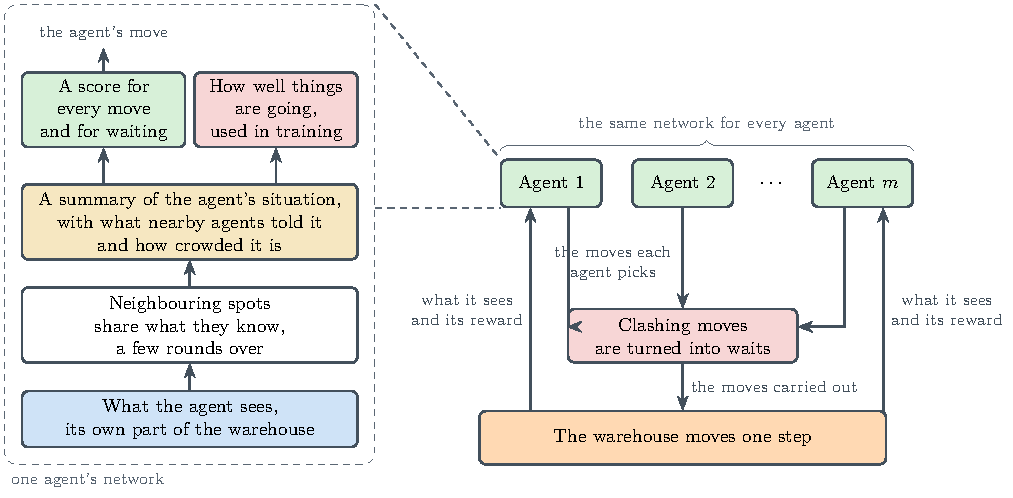
\includegraphics[width=\linewidth]{old_architecture.pdf}\\[-2pt]{\small stays: \texttt{fig:architecture}}
\end{minipage}\hfill
\begin{minipage}{0.47\linewidth}\centering
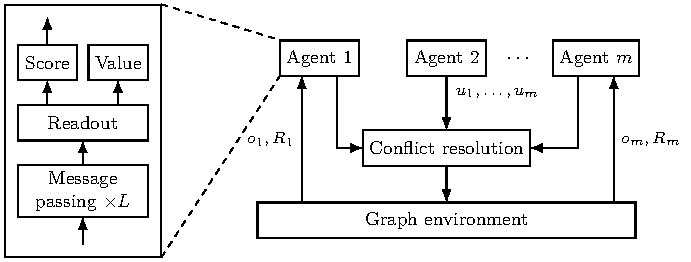
\includegraphics[width=0.8\linewidth]{old_architecture_compact.pdf}\\[-2pt]{\small moves to Appendix C}
\end{minipage}
\end{center}

\textbf{Implementation, ``How an agent chooses its move''.} \ldots{} and adds messages between agents
as in Pham et al. Appendix~\texttt{app:controllers:sources} sets the three side by side\new{ and
draws the model in the form of their figure.}\old{, and Figure~\texttt{architecturecompact} draws
the model in the form of their figure.} \mockup{The figure block of \texttt{architecture\_compact.pdf}
is removed here.}

\textbf{Appendix C, ``The model against its sources'', after the paragraph on graph convolution.}
\new{Figure~\texttt{architecturecompact} draws the model in the form of Figure~3 of van Knippenberg
et al. The move score, the value head and conflict resolution are what this model adds.}
\mockup{The figure, label \texttt{fig:architecturecompact} kept, caption ``The model drawn as
Figure~3 of van Knippenberg et al.''}

\subsection*{2.2 The same three panels twice (Problem Formulation)}
\begin{center}
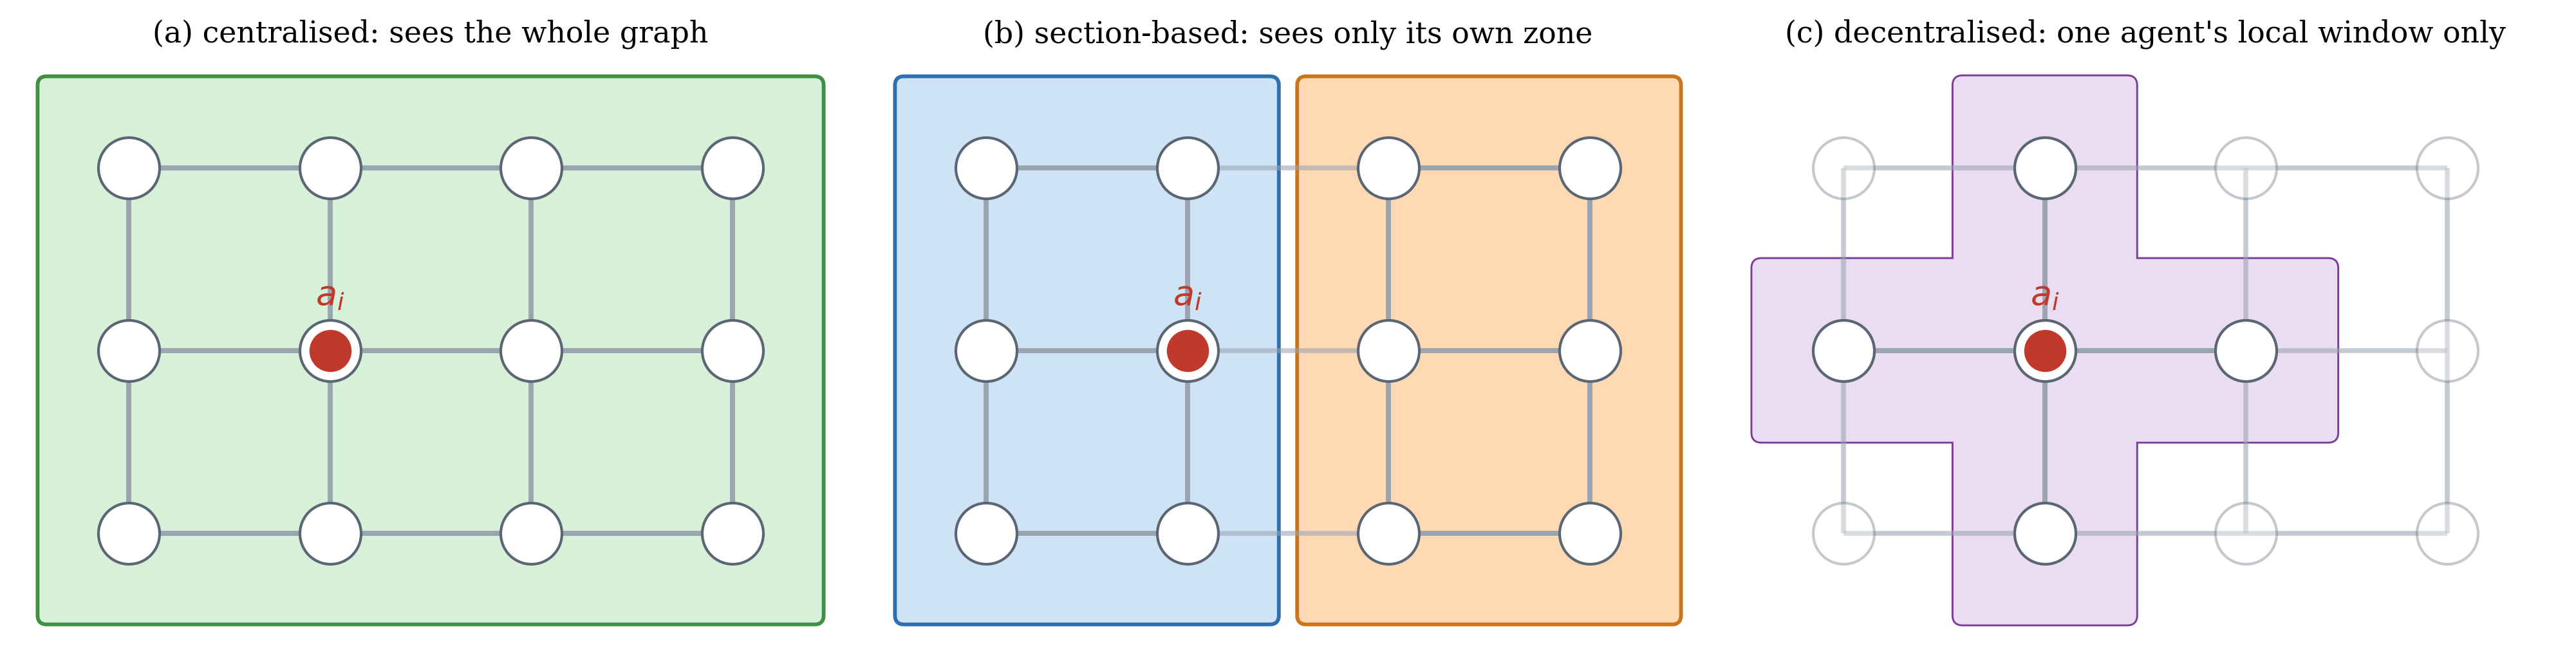
\includegraphics[width=\linewidth]{old_controllers_example.png}\\{\small before, \texttt{fig:controllers-example}}\\[6pt]
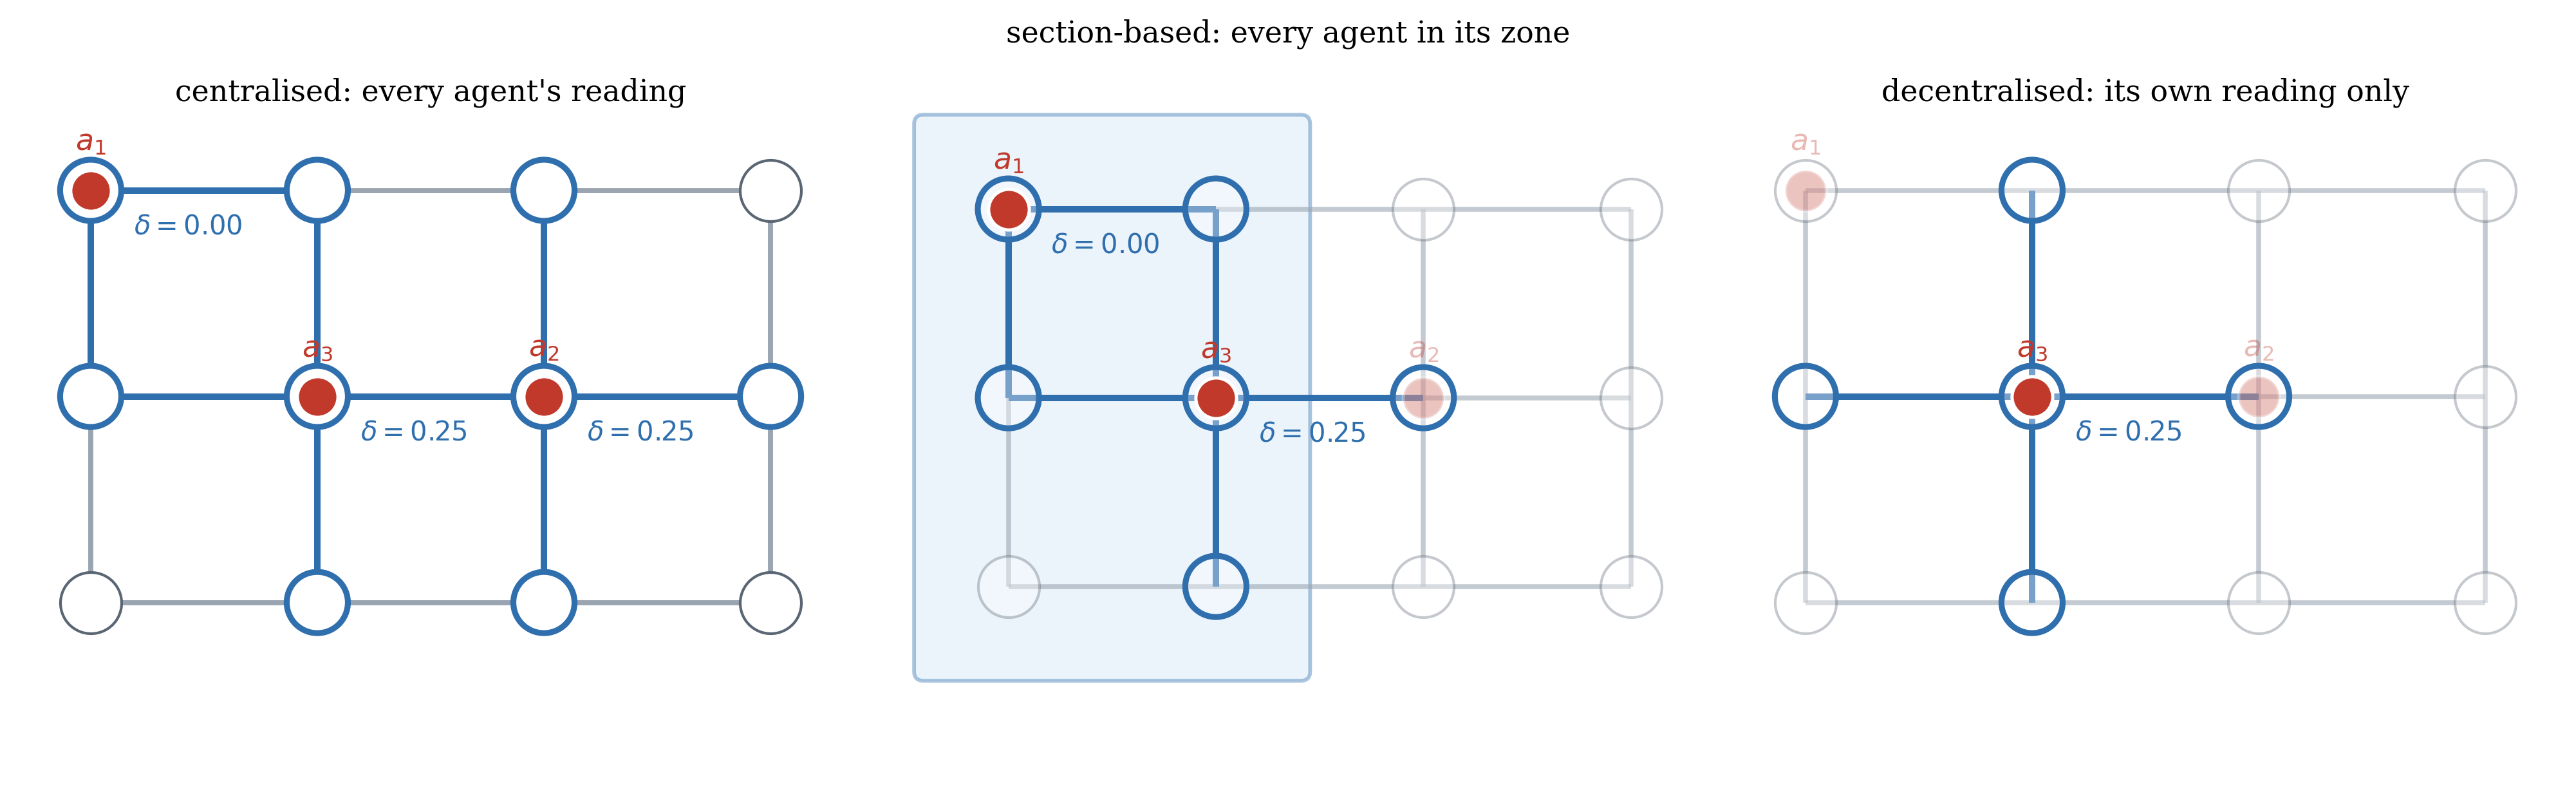
\includegraphics[width=\linewidth]{old_congestion_mini.png}\\{\small before, \texttt{fig:congestion}}\\[6pt]
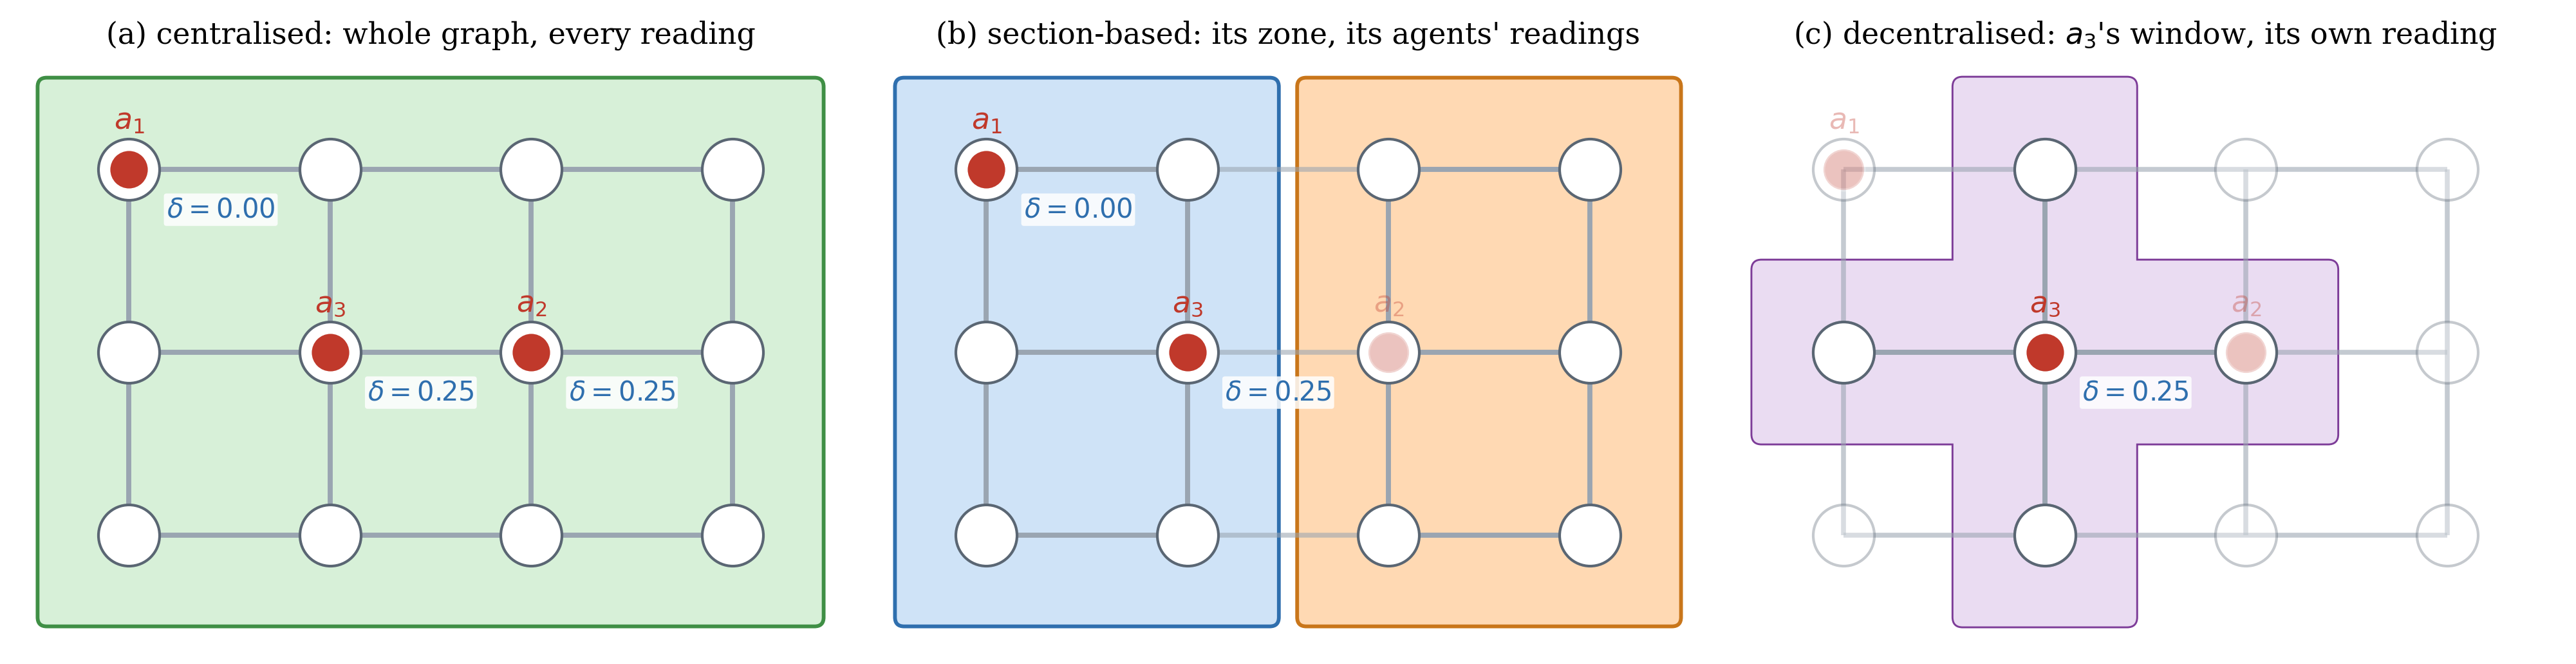
\includegraphics[width=\linewidth]{controllers_window_new.png}\\{\small after, one figure, \texttt{fig:controllers-example}}
\end{center}

\textbf{``Who decides'', where the figure stands now.} \mockup{The figure is
\texttt{controllers\_window.png}.} Caption: \new{The same small graph under each architecture's
window. Each panel writes the crowding feature $\delta$ of Section~\texttt{pf:observations} beside
the agents its controller decides for.} \old{Faded vertices are outside the controller's window.}

\textbf{``How crowded the neighbourhood is''.} \ldots{} explains why a section-based agent's field
of view is not cut at the zone edge. \new{Figure~\texttt{controllers-example} gives each agent's
reading, beside the agents each controller decides for.} \old{Figure~\texttt{congestion} shows the
same field of view for every agent, on the graph of Figure~\texttt{controllers-example}.}
\mockup{The figure block of \texttt{congestion\_mini.png} is removed.}

\textbf{Two more references} to \texttt{fig:congestion} point to \texttt{fig:controllers-example}
instead: the loop section (``the crowding feature of Figure~\ldots'') and ``Crowding'' (``In the
centralised panel of Figure~\ldots{} the three agents read 0, 0.25 and 0.25''). The values are the
same in the new figure.

\subsection*{2.3 The tea example (Problem Formulation, ``What the rule decides'')}
\begin{center}
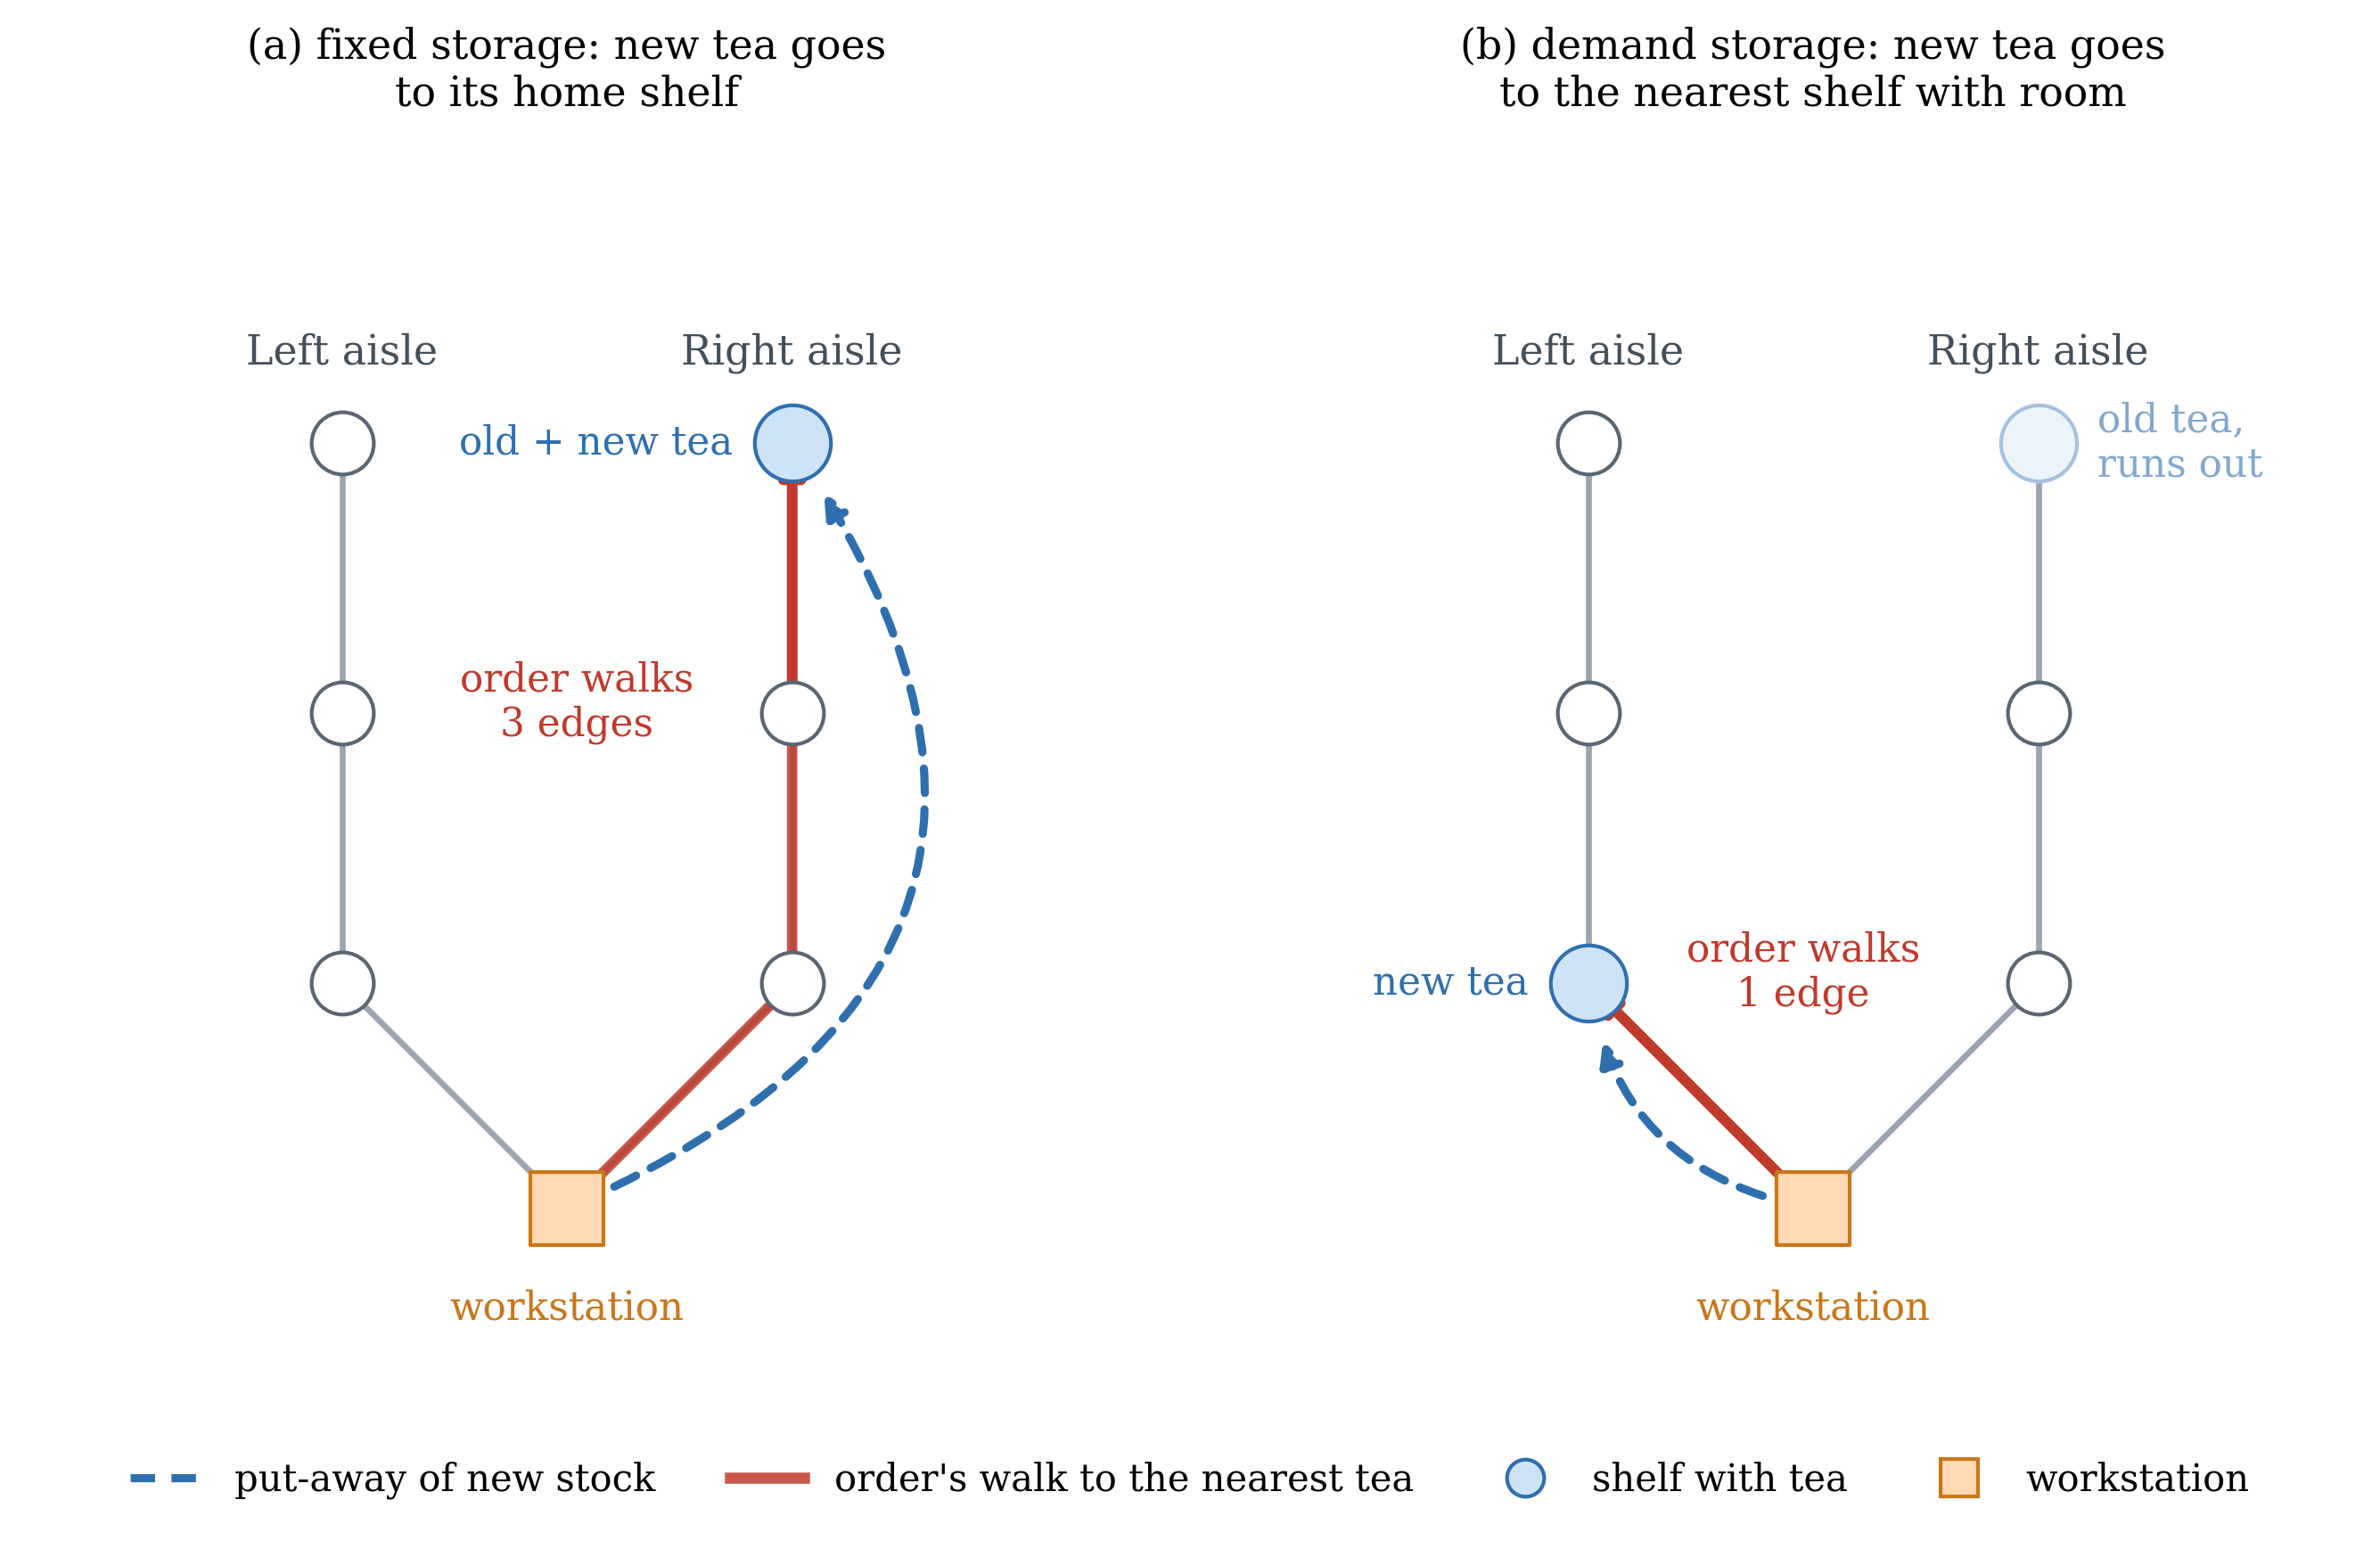
\includegraphics[width=0.75\linewidth]{old_arrival_storage.png}\\{\small before}\\[6pt]
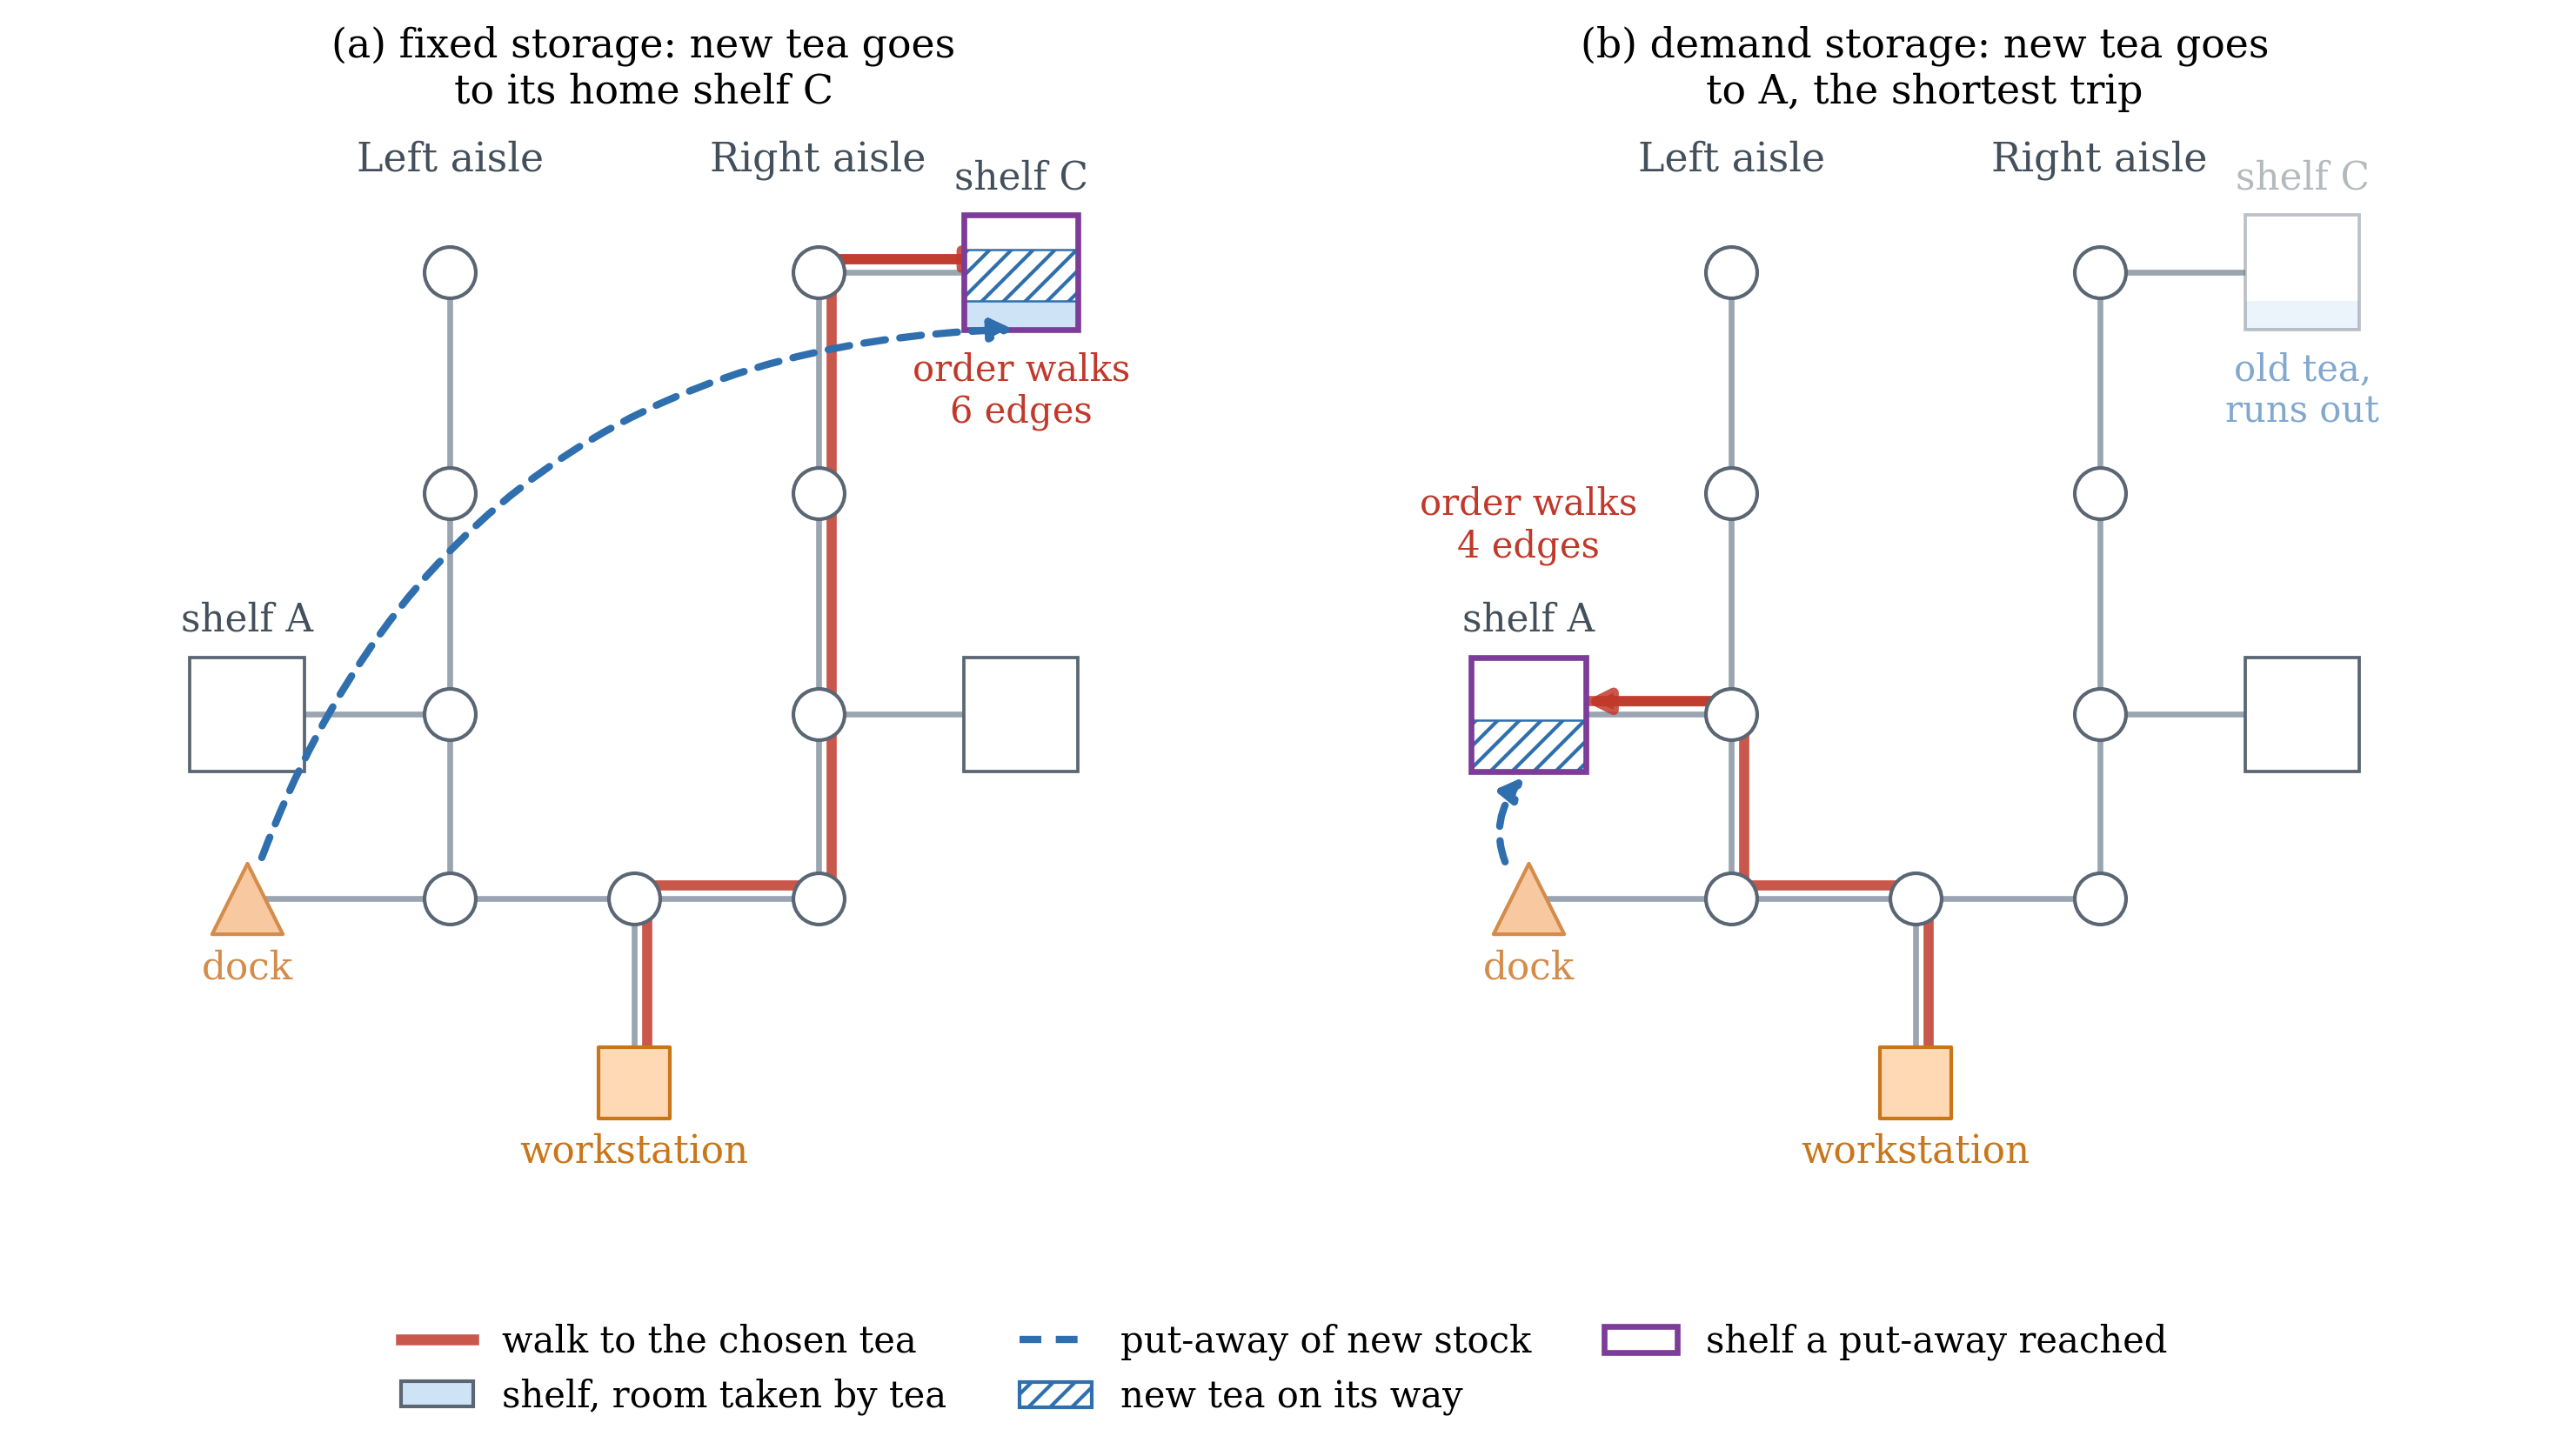
\includegraphics[width=0.85\linewidth]{arrival_storage_new.png}\\{\small after, \texttt{fig:storageexample}}
\end{center}

Figure~\texttt{storageexample} shows tea that has become popular. Under fixed storage, new tea goes
back to its home shelf\new{ C, and an order walks six edges to it from the workstation.}\old{,
three edges from the workstation.} Under demand storage, it goes to \new{shelf A, the shortest trip
from the dock to the workstation, and an order walks four edges.}\old{the nearest shelf with room,
one edge away.} The old tea stays where it is and runs down as it is picked.

Caption, unchanged: Arriving tea under fixed and demand storage. Old tea stays where it is, so only
the new tea's shelf differs.

\subsection*{2.4 The loop figure, dock moved (Problem Formulation, the loop)}
\begin{center}
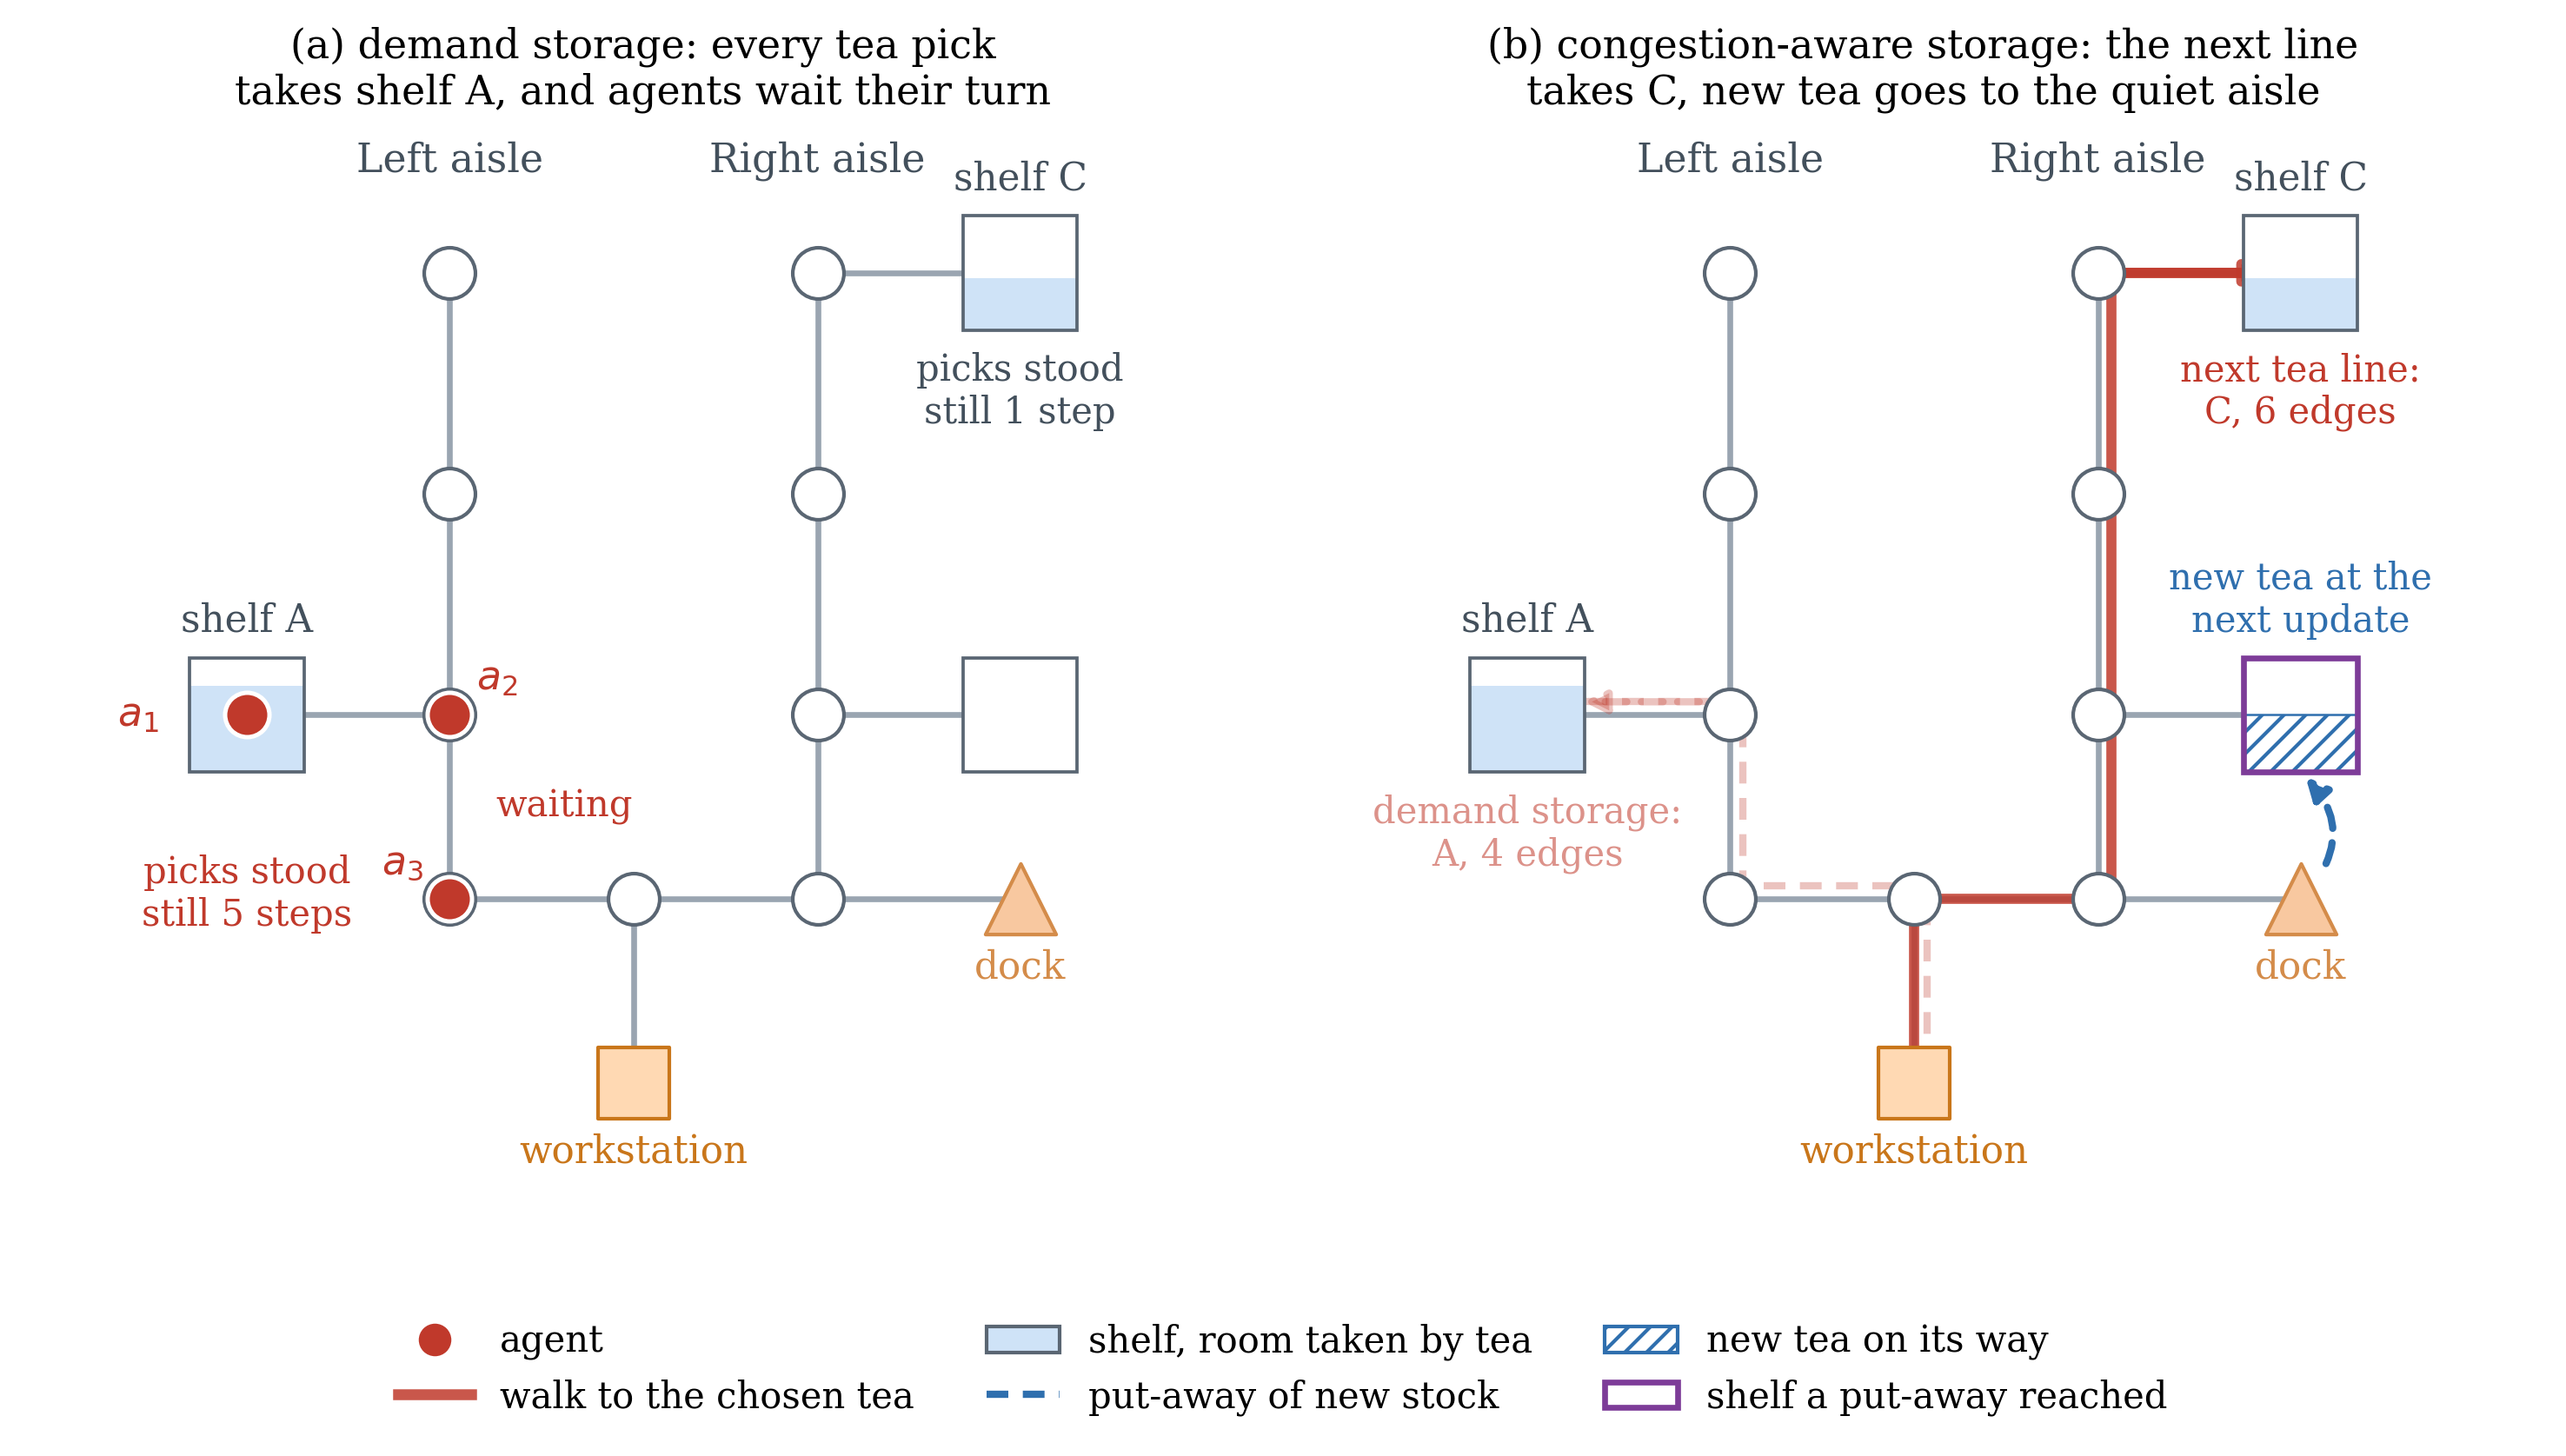
\includegraphics[width=0.75\linewidth]{old_shelf_loop.png}\\{\small before}\\[6pt]
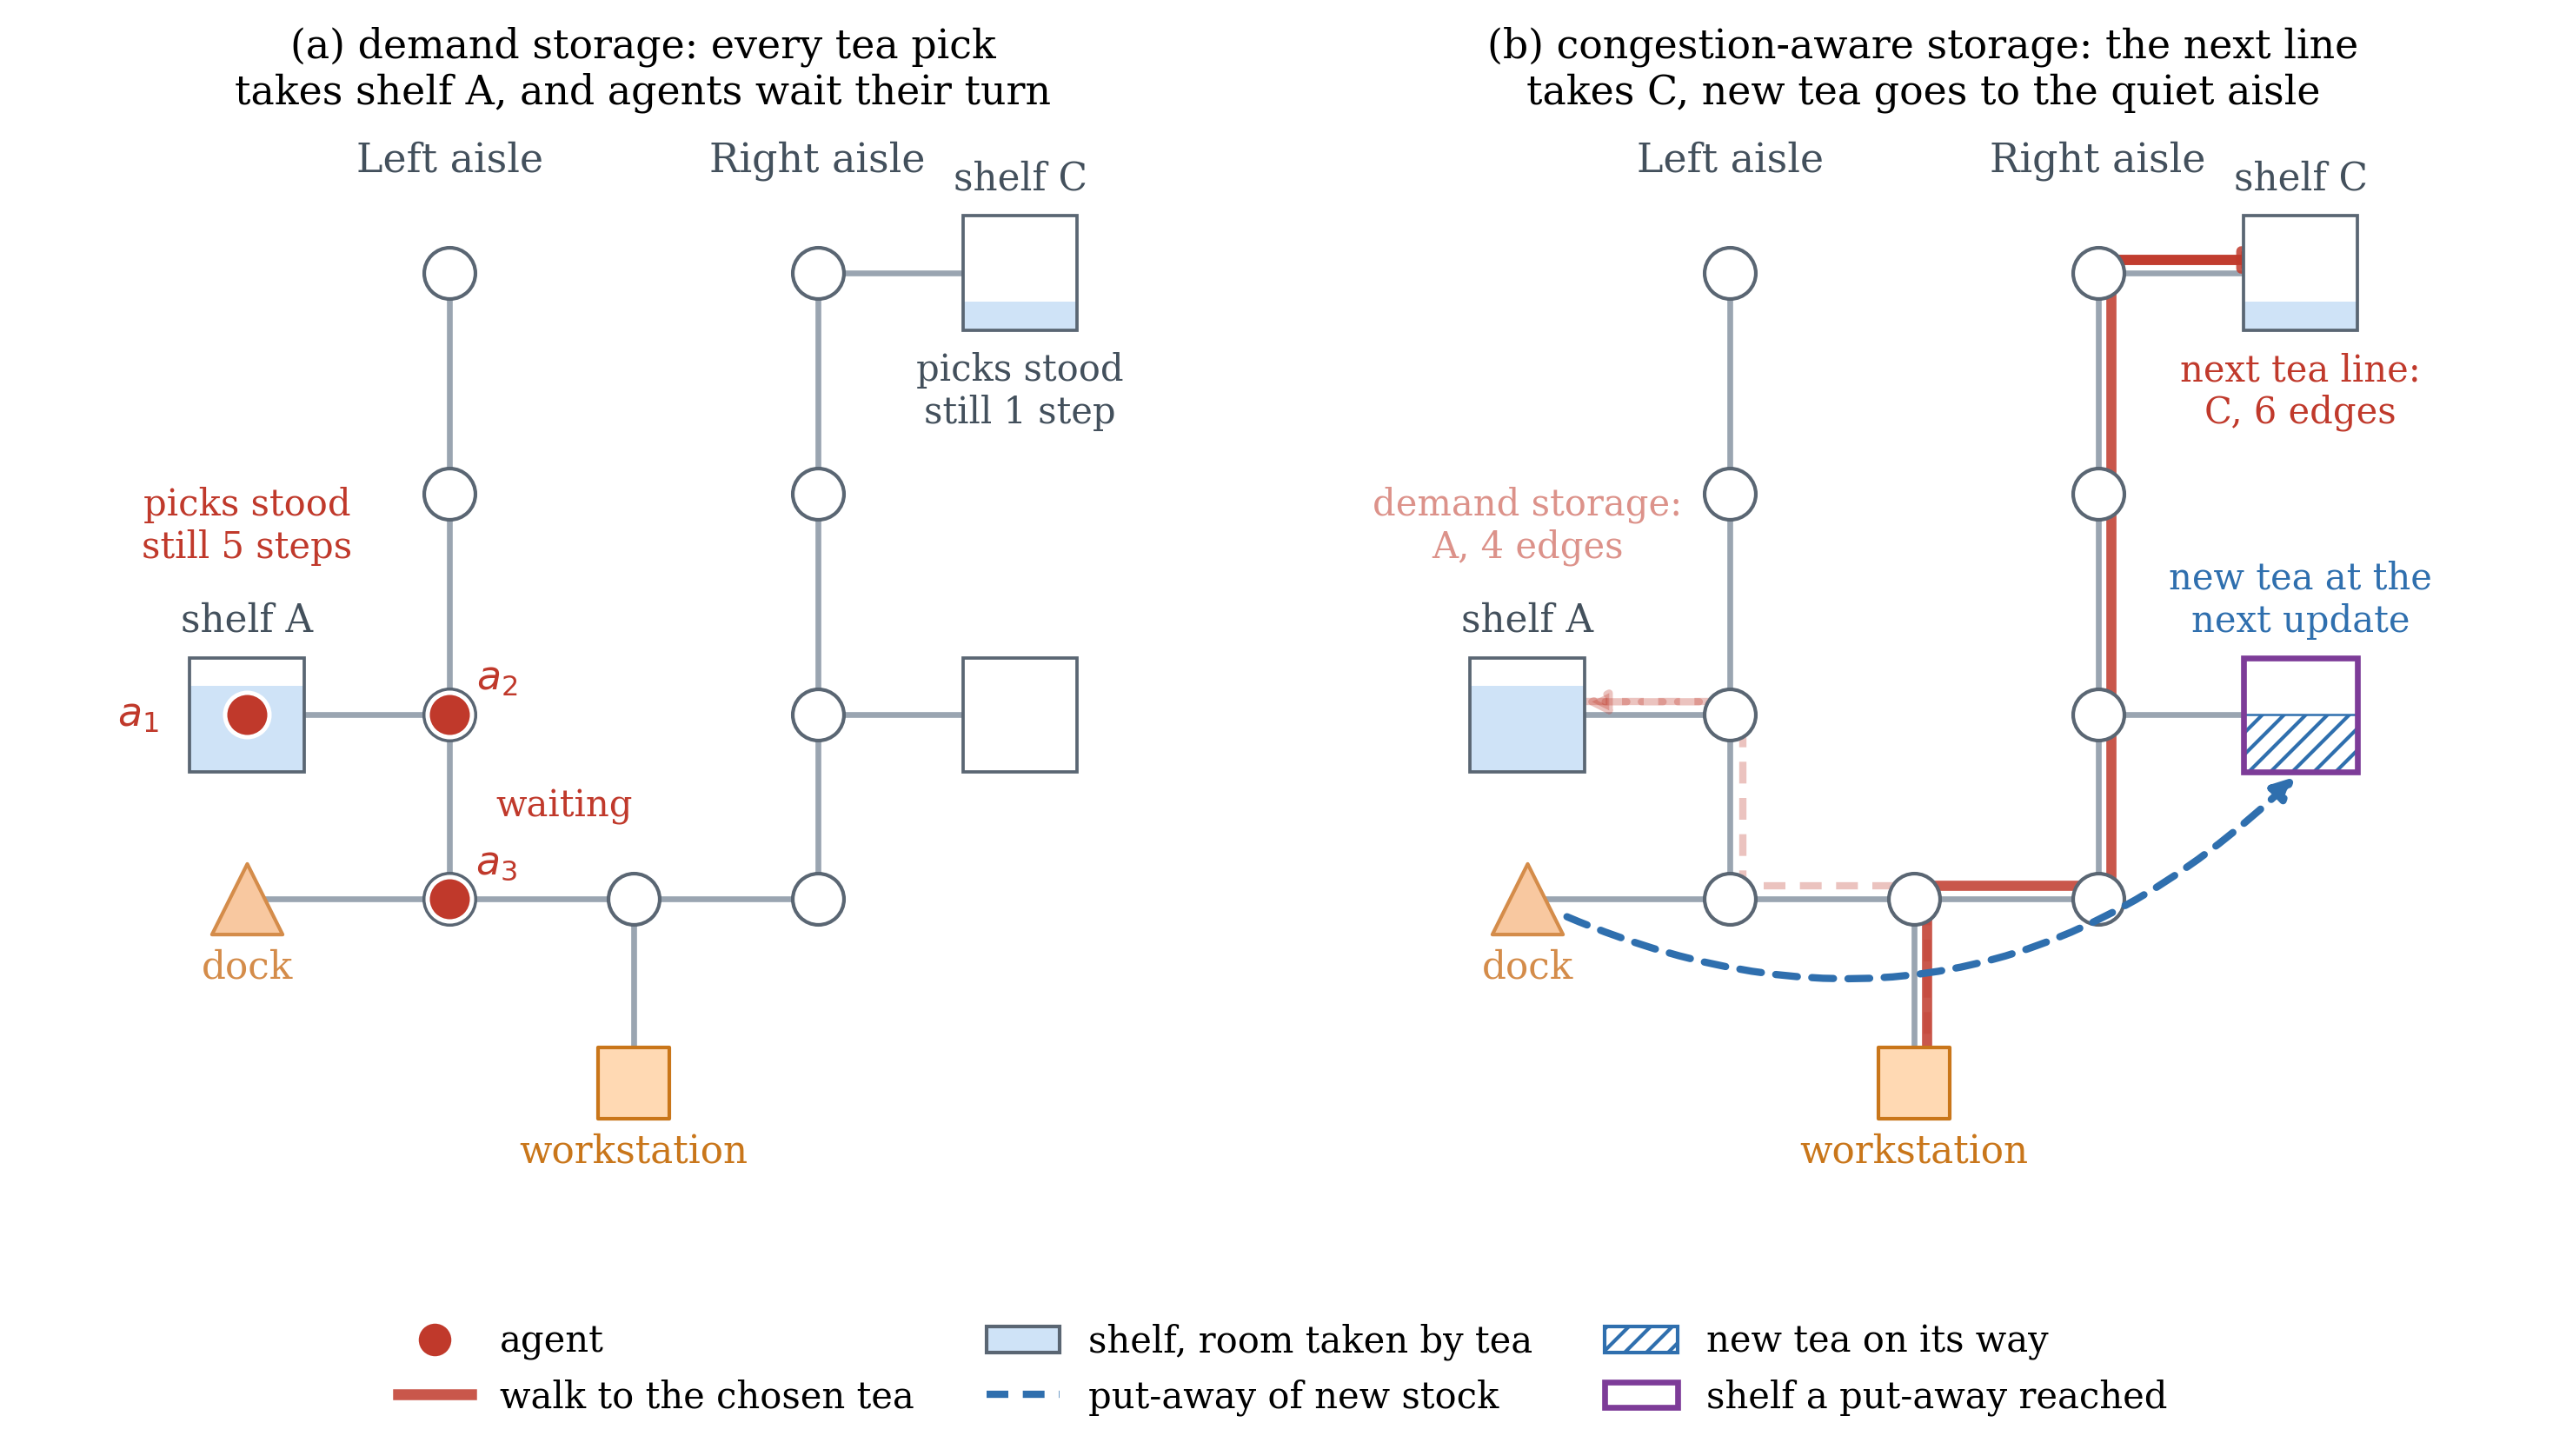
\includegraphics[width=0.85\linewidth]{shelf_loop_new.png}\\{\small after, \texttt{fig:loop}}
\end{center}
\mockup{The text and caption stay. Only the dock moves to the left, and with it the put-away arrow.}

\section*{Part 3. Questions}
\begin{enumerate}[leftmargin=1.4em]
\item \textbf{Where the merged figure stands.} It stays in ``Who decides'', where the windows are
  first needed. It shows $\delta$ about 200 lines before $\delta$ is explained, so the caption points
  ahead to it. The other place is ``How crowded the neighbourhood is'', where $\delta$ is
  introduced. Then ``Who decides'' has only Table~\texttt{information} for the windows. Which?
\item \textbf{The compact model figure in Appendix C.} Moved as it is, or dropped altogether, since
  Appendix C already writes the three sources side by side in equations?
\item \textbf{The tea example's numbers.} The text now gives the walks as six and four edges, from
  the new figure. Keep the numbers in the text, or leave them to the figure?
\end{enumerate}

\end{document}
